\section{The Bag-of-Tasks Pattern}

In the previous sections, we chose to distribute the work equally between the
workers.
%
This is sensible if each worker will be executed on its own processor,
all the processors are the same speed, all are equally loaded with other
tasks, and it's possible to identify what an equal distribution is.
%
But in many cases, not all of these things will be true.

An alternative is to use smaller tasks, with more tasks than workers.  
%
In the numerical integration example, each task will be to estimate the
integral over some subrange.   We use \SCALA{nTasks} tasks, where
$\sm{nTasks} \ge \sm{nWorkers}$.
%
The tasks are distributed between the workers, each receiving a new task when
it has finished the previous one.  In this way, the faster workers will
complete more tasks than the slower ones, which provides for a form of load
balancing.

This pattern is known as \emph{bag of tasks}: the controller holds a bag of
tasks, which it distributes to workers.  (Sometimes workers return sub-tasks
to the controller, but that's not the case here.)

%%%%%

Most of the code to apply the bag-of-tasks pattern to the numerical
integration example is in Figure~\ref{fig:bag-of-tasks}.  (We omit code that
is essentially identical to earlier.)

Adapting the definition of a worker is straightforward.  Each worker thread
repeatedly receives and processes tasks, keeping track of the sum of the
estimates it has calculated so far.  
%
The controller closes the |toWorkers| channel to indicate that there are no
remaining tasks, at which point the worker sends its total to the controller.
%
An alternative would be to send the subresult for each task to the controller
immediately; however, that would lead to more channel communications, so is
likely to be slower.

%%%%%%%%%%%%%%%%%%%%%%%%

\begin{figure}
\begin{scala}
  private def worker = thread("worker"){
    var myTotal = 0.0
    repeat{
      val (left, right, taskSize, delta) = toWorkers?()
      myTotal += integral(left, right, taskSize, delta)
    }
    toController!myTotal
  }

  private def distributor = thread("distributor"){
    val delta = (b-a)/n    // Size of each interval.
    var remainingIntervals = n    // Number of intervals not yet allocated.
    var left = a // Left-hand boundary of next task.
    for(i <- 0 until nTasks){
      // Number of intervals in the next task; £$\lceil \sm{remainingIntervals}/(\sm{nTasks}-\sm i)\rceil$£.
      val taskSize = ((remainingIntervals-1) / (nTasks-i) + 1).toInt
      remainingIntervals -= taskSize; val right = left+taskSize*delta
      toWorkers!(left, right, taskSize, delta); left = right
    }
    toWorkers.endOfStream()
  }

  private var result = 0.0

  private def collector = thread("collector"){
    result = 0.0
    for(i <- 0 until nWorkers) result += toController?()
  }

  private def system = {
    val workers = || (for (i <- 0 until nWorkers) yield worker)
    workers || distributor || collector
  }

  def apply(): Double = { run(system); result } 
\end{scala}
\caption{The bag-of-tasks pattern applied to the numerical integration
  example.}
\label{fig:bag-of-tasks}
\end{figure}

%%%%%%%%%%


%%%%% \heading{The controller}

The controller has to both distribute tasks (on |toWorkers|), and receive
results (on |toController|).
%
We could implement this using a single controller thread.  This approach would
be reasonably straightforward in this case, because all the communications on
|toController| follow those on |toWorkers|.  However, in other examples the
communications over the different channels might be interleaved, which makes a
single-thread approach trickier.

The issues of distributing the tasks and receiving the results are
independent, so it is cleaner to separate them.  The easiest way to do this is
to use two concurrent threads, one for each aspect.  In some examples, this
might also give better performance, if the controller acts as a bottleneck.

We therefore build the controller as the composition of a distributor and a
collector, communicating with the workers as illustrated below.
%
\begin{center}
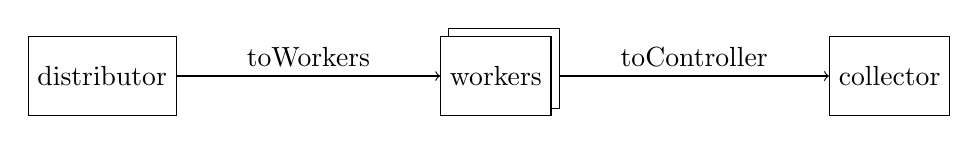
\begin{tikzpicture}
\draw (0,0) node[draw, minimum height = 10mm](d){\scalashape distributor};
\draw (5,0) node[draw, minimum height = 10mm] (w){\scalashape workers};
\draw ([xshift = 1mm] w.north west) -- ++ (0,1mm) -- 
  ([xshift = 1mm, yshift = 1mm] w.north east) -- 
  ([xshift = 1mm, yshift = 1mm] w.south east) -- 
  ([yshift = 1mm] w.south east) ;
\draw[->] (d) -- node[above]{\scalashape toWorkers}   (w);
%
\draw (10,0)  node[draw, minimum height = 10mm](c){\scalashape collector};
\draw[->] ([xshift = 1mm] w.east) -- node[above]{\scalashape toController} (c);
\end{tikzpicture}
\end{center}

%%%%%

The code for distributing the tasks is almost identical to earlier, except now
the distributor sends out |nTasks| tasks.  And the code for the collector is
identical to the relevant part of the previous controller. 

We then construct the system as illustrated above.  The resulting program can
be tested in the same way as for the previous implementation. 

\begin{instruction}
Study the details of the implementation.
\end{instruction}
